\documentclass[11pt,twoside,a4paper]{article}
% http://www-h.eng.cam.ac.uk/help/tpl/textprocessing/latex_maths+pix/node6.html symboles de math
% http://fr.wikibooks.org/wiki/Programmation_LaTeX Programmation latex (wikibook)
%=========================== En-Tete =================================
%--- Insertion de paquetages (optionnel) ---
\usepackage[french]{babel}   % pour dire que le texte est en fran{\'e}ais
\usepackage{a4}	             % pour la taille   
\usepackage[T1]{fontenc}     % pour les font postscript
\usepackage{epsfig}          % pour gerer les images
%\usepackage{psfig}
\usepackage{amsmath, amsthm} % tres bon mode mathematique
\usepackage{amsfonts,amssymb}% permet la definition des ensembles
\usepackage{float}           % pour le placement des figure
\usepackage{verbatim}

\usepackage{longtable} % pour les tableaux de plusieurs pages

\usepackage[table]{xcolor} % couleur de fond des cellules de tableaux

\usepackage{lastpage}

\usepackage{multirow}

\usepackage{multicol} % pour {\'e}crire dans certaines zones en colonnes : \begin{multicols}{nb colonnes}...\end{multicols} 

% \usepackage[top=1.5cm, bottom=1.5cm, left=1.5cm, right=1.5cm]{geometry}
% gauche, haut, droite, bas, entete, ente2txt, pied, txt2pied
\usepackage{vmargin}
\setmarginsrb{0.20cm}{0.20cm}{0.20cm}{0.20cm}{15pt}{3pt}{15pt}{3pt}

\usepackage{lscape} % changement orientation page
%\usepackage{frbib} % enlever pour obtenir references en anglais
% --- style de page (pour les en-tete) ---
\pagestyle{empty}

% % % en-tete et pieds de page configurables : fancyhdr.sty

% http://www.trustonme.net/didactels/250.html

% http://ww3.ac-poitiers.fr/math/tex/pratique/entete/entete.htm
% http://www.ctan.org/tex-archive/macros/latex/contrib/fancyhdr/fancyhdr.pdf
% \usepackage{fancyhdr}
% \pagestyle{fancy}
% % \newcommand{\chaptermark}[1]{\markboth{#1}{}}
% % \newcommand{\sectionmark}[1]{\markright{\thesection\ #1}}
% \fancyhf{}
% \fancyhead[LE,RO]{\bfseries\thepage}
% \fancyhead[LO]{\bfseries\rightmark}
% \fancyhead[RE]{\bfseries\leftmark}
% \fancyfoot[LE]{\thepage /\pageref{LastPage} \hfill
	% TITLE
% \hfill 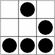
\includegraphics[width=0.5cm]{img/logo_glider.png} }
% \fancyfoot[RO]{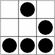
\includegraphics[width=0.5cm]{img/logo_glider.png} \hfill
	% TITLE
% \hfill \thepage /\pageref{LastPage}}
% \renewcommand{\headrulewidth}{0.5pt}
% \renewcommand{\footrulewidth}{0.5pt}
% \addtolength{\headheight}{0.5pt}
% \fancypagestyle{plain}{
	% \fancyhead{}
	% \renewcommand{\headrulewidth}{0pt}
% }


%============================= Corps =================================
\begin{document}

\setlength\parindent{0pt}

\texttt{http://rue89.nouvelobs.com/2014/12/21/wikileaks-revele-les-astuces-cia-passer-les-frontieres-sans-faire-choper-256635}~\\

\textbf{\LARGE WikiLeaks r{\'e}v{\`e}le les astuces de la CIA pour passer les fronti{\`e}res sans se faire choper} ~\\

\emph{\small par Jean-Marc Manach | Journaliste, Fuite 21/12/2014 {\`a} 19h01} ~\\

\textbf{Des documents de la CIA que r{\'e}v{\`e}lent WikiLeaks et Rue89 listent les conseils pratiques de l'agence am{\'e}ricaine {\`a} destination de ses espions pour passer sans souci les contr{\^o}les de s{\'e}curit{\'e} des a{\'e}roports. } ~\\

%% \begin{minipage}[ht]{7.00cm}
%% 	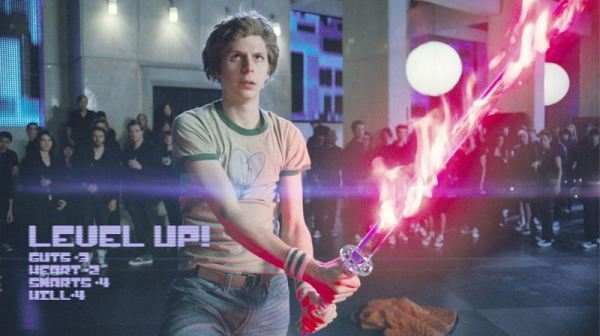
\includegraphics[width=6.95cm]{img/59580392.jpg}
%% \end{minipage} \hfill \begin{minipage}[ht]{0.65\textwidth}
%% 	Un paragraphe accompagn{\'e} d'une image. %% ~\\
%% \end{minipage}~\\~\\

%% \textbf{\large Un sous-titre}~\\

Contrairement {\`a} ce qu'on peut \texttt{lire}~\footnote{\texttt{https://en.wikipedia.org/wiki/Lithium-ion\_battery\#History}} sur Wikip{\'e}dia, la batterie au lithium-ion, qui a notamment contribu{\'e} {\`a} l'expansion des smartphones et ordinateurs portables, aurait {\'e}t{\'e} invent{\'e}e par la \texttt{Direction de la science et de la technologie}~\footnote{\texttt{https://www.cia.gov/fr/offices-of-cia/science-technology/index.html}} (DS\&T) de la CIA. ~\\

Initialement con\c{c}ue pour \texttt{prolonger la dur{\'e}e de vie}~\footnote{\texttt{http://www.cia.gov/news-information/featured-story-archive/2010-featured-story-archive/dst-innovations-lithium-iodine-battery.html}} de certains satellites et syst{\`e}mes de surveillance, la CIA en aurait confi{\'e} les secrets {\`a} des m{\'e}decins, aux d{\'e}buts des ann{\'e}es 70, afin qu'ils s'en servent pour alimenter des pacemakers, avant que son usage ne se g{\'e}n{\'e}ralise avec le succ{\`e}s que l'on sait. ~\\

A en croire la CIA, ce que font les petits g{\'e}nies de sa DS\&T serait \texttt{<<encore plus impressionnant>>}~\footnote{\texttt{https://www.cia.gov/news-information/featured-story-archive/directorate-of-science-and-technology.html}} que ce que fait Q dans <<James Bond>>. \texttt{Elle se vante}~\footnote{\texttt{http://www.cia.gov/news-information/featured-story-archive/2014-featured-story-archive/the-cia-and-you-cia2019s-contributions-to-modern-technology.html}} ainsi d'avoir d{\'e}velopp{\'e}, d{\`e}s les ann{\'e}es 70, le premier drone de la taille d'une libellule, ou encore une technologie d'analyse d'images satellitaires qui, utilis{\'e}e depuis pour d{\'e}tecter le cancer du sein, aurait consid{\'e}rablement r{\'e}duit la mortalit{\'e} en la mati{\`e}re, mais aussi permis aux utilisateurs de Google Earth de pouvoir zoomer sur la quasi-totalit{\'e} des points du globe. ~\\

%% Vid{\'e}o de la CIA intitul{\'e}e <<L'impact de la CIA sur la technologie>>

Entre autres missions, la DS\&T est \texttt{charg{\'e}e}~\footnote{\texttt{https://www.cia.gov/fr/offices-of-cia/science-technology/}} d'aider la CIA lorsqu'elle est confront{\'e}e {\`a} des probl{\`e}mes <<durant l'acquisition de renseignements clandestins>>, de fournir <<des modes de communication s{\'e}curis{\'e}s>> {\`a} ses agents, ainsi que des syst{\`e}mes et outils de <<surveillances audio et vid{\'e}o>> . ~\\

WikiLeaks, qui avait \texttt{rendu public}~\footnote{\texttt{https://wikileaks.org/cia-hvt-counterinsurgency/press-release.html}} il y a quelques jours un m{\'e}mo de la CIA sur son programme d'assassinats cibl{\'e}s, \texttt{r{\'e}v{\`e}le aujourd'hui}~\footnote{\texttt{http://wikileaks.org/cia-travel/}}, en partenariat avec Rue89 et quelques autres m{\'e}dias, deux autres de ses manuels. ~\\

Classifi{\'e}s <<Secret/\texttt{NoForn}~\footnote{\texttt{https://en.wikipedia.org/wiki/Classified\_information\_in\_the\_United\_States\#Handling\_caveats}}>> (pour N<<o Foreign National Access Allowed>>, dont l'acc{\`e}s est donc interdit aux non-Am{\'e}ricains), ils {\'e}manent de Checkpoint, l'une des structures de la DS\&T, qui n'avait jusqu'alors jamais fait parler d'elle. ~\\

%% Voir le document (Fichier PDF)

Checkpoint est charg{\'e}e de collecter, analyser et diss{\'e}miner les informations susceptibles de prot{\'e}ger l'identit{\'e} et les activit{\'e}s des agents de la CIA lorsqu'ils voyagent {\`a} l'{\'e}tranger. --- Les documents ne pr{\'e}cisent pas si Checkpoint fournit aussi de faux documents de voyage ou d'identit{\'e} aux espions am{\'e}ricains. ~\\

Ils r{\'e}v{\`e}lent par contre les m{\'e}thodes, trucs et astuces qu'ils utilisent pour passer les contr{\^o}les aux fronti{\`e}res dans les a{\'e}roports internationaux sans se faire rep{\'e}rer, et <<survivre>> (sic) aux {\'e}ventuels contr{\^o}les renforc{\'e}s dont ils pourraient faire l'objet, ainsi que les pratiques et m{\'e}thodes utilis{\'e}es par certaines forces de s{\'e}curit{\'e}, {\`a} l'{\'e}tranger, pour identifier les <<suspects>> {\`a} interroger. ~\\

Vous voulez {\'e}viter de vous faire attraper par la police aux fronti{\`e}res ? Suivez les conseils de la CIA. ~\\

\textbf{\large 1 -- N'achetez pas votre billet d'avion en liquide et n'oubliez pas d'enregistrer des bagages}~\\

Le premier document, datant de septembre 2011, commence par rappeler que les citoyens am{\'e}ricains d{\'e}tenteurs de passeports diplomatiques ne sont pas des Am{\'e}ricains comme les autres. ~\\

En effet, si 50 pays exigent des d{\'e}tenteurs de passeports am{\'e}ricains qu'ils demandent un visa, 120 pays le font d{\`e}s lorsqu'ils s'agit de passeports diplomatiques. ~\\

Nombreux sont en effet les espions agissant sous couverture diplomatique, faisant de tout employ{\'e} de l'administration ou de l'arm{\'e}e US un <<suspect>> en puissance, a fortiori dans les pays qui, {\`a} l'instar de la Georgie, du Pakistan, de la Russie ou de l'Ouzbekhistan, font valider les demandes de visa par leurs services de renseignement. ~\\

Au-del{\`a} des demandes de visa, la CIA rappelle que les probl{\`e}mes commencent avant m{\^e}me de prendre l'avion :
\begin{itemize}
	\item le fait de payer son billet en liquide ;
	\item de l'acheter au sein m{\^e}me de l'a{\'e}roport, ou la veille du d{\'e}part ;
	\item pour un aller simple ;
	\item et sans bagage enregistr{\'e}, pourrait ainsi vous valoir un interrogatoire.
\end{itemize}

C'est, {\`a} en croire le rapport, ce que font par exemple les services anti-immigration sud-africains, et ce qu'auraient d{\^u} faire les autorit{\'e}s n{\'e}erlandaises {\`a} Noël 2009, ce qui leur aurait permis d'emp{\^e}cher le <<terroriste au slip>> d'embarquer dans un avion {\`a} destination de Detroit (heureusement, sa bombe \texttt{n'avait pas explos{\'e}}~\footnote{\texttt{http://rue89.nouvelobs.com/2009/12/26/attentat-manque-a-detroit-la-menace-du-terrorisme-amateur-131323}}, et il avait {\'e}t{\'e} ceintur{\'e} par d'autres passagers). ~\\

\textbf{\large 2 -- Evitez d'{\^e}tre fich{\'e} (l'enfance de l'art)}~\\

A l'image de ce qu'avaient impos{\'e} les Etats-Unis {\`a} toutes les compagnies a{\'e}riennes d{\'e}sirant pouvoir atterrir sur (ou transiter par) son territoire, suite aux attentats de septembre 2001, un nombre croissant de pays exigent de recevoir les donn{\'e}es d{\'e}taill{\'e}es des dossiers passagers (ou \texttt{PNR}~\footnote{\texttt{https://fr.wikipedia.org/wiki/Passenger\_Name\_Record}}, pour <<Passenger Name Record>>) de ceux qui prennent l'avion (noms, itin{\'e}raires, voire r{\'e}servations d'h{\^o}tel ou de voitures, pr{\'e}f{\'e}rences alimentaires -- casher, hallal –, etc.). ~\\

L'objectif est de les comparer, notamment, aux <<listes noires>> de ceux qui sont interdits de territoire, et d'identifier de potentiels suspects, quitte {\`a} interdire {\`a} l'avion d'atterrir, ou {\`a} le d{\'e}router. --- Si la majeure partie de ces <<listes noires>> concernent des terroristes pr{\'e}sum{\'e}s, criminels recherch{\'e}s ou des migrants expuls{\'e}s, d'apr{\`e}s <<plusieurs sources clandestines>> cit{\'e}es dans le rapport, elles peuvent aussi viser les agents (confirm{\'e}s ou suspect{\'e}s) de services de renseignement {\'e}trangers. ~\\

L'Autriche et Singapour cibleraient ainsi les espions russes, la Colombie, les Iraniens et les V{\'e}n{\'e}zu{\'e}liens, le Tadjikistan, les agents de <<plusieurs pays occidentaux non identifi{\'e}s>>, tandis que la Hongrie regarderait de pr{\`e}s les d{\'e}tenteurs de billets d'avion, r{\'e}servations d'h{\^o}tel ou de voiture de location achet{\'e}s par une centrale d'achat gouvernementale ou militaire. ~\\

\textbf{\large 3 -- Gare aux ordinateurs et aux cigarettes {\'e}lectroniques}~\\

Les espions, les terroristes, les criminels et les sans-papiers ne sont pas les seuls {\`a} b{\'e}n{\'e}ficier de l'attention des services de s{\'e}curit{\'e}. --- A l'a{\'e}roport international Imam-Khomeini, en Iran, toute personne trouv{\'e}e en possession de photos ou vid{\'e}os de manifestations -- ou de toute activit{\'e} {\'e}voquant l'opposition -- fait ainsi l'objet d'une fouille approfondie de son ordinateur et de tous ses appareils {\'e}lectroniques. --- A l'a{\'e}roport international de Bahre{\"i}n, la simple possession d'un <<ustensile {\'e}lectronique insolite>> implique un interrogatoire de s{\'e}curit{\'e} pouss{\'e}. Avis aux utilisateurs de cigarettes {\'e}lectroniques, bracelets connect{\'e}s et autres objets <<branch{\'e}s>>... ~\\

\textbf{\large 4 -- Sachez quel pays est capable ou non d'authentifier un passeport biom{\'e}trique}~\\

Le rapport s'{\'e}tonne de d{\'e}couvrir que plusieurs pays d{\'e}livrant des passeports biom{\'e}triques ne v{\'e}rifiaient pas qu'ils avaient correctement {\'e}t{\'e} sign{\'e}s, et qu'ils n'avaient donc pas {\'e}t{\'e} falsifi{\'e}s... ~\\

Au dernier pointage, en mai 2014, une trentaine de pays (dont l'Italie, la Pologne, la Finlande, l'Estonie, l'Alg{\'e}rie, le S{\'e}n{\'e}gal, le Ghana, le Cambodge, Singapour, l'Indon{\'e}sie ou le Chili) ne participaient toujours pas au programme d'authentification des passeports biom{\'e}triques, quand bien m{\^e}me ils ont pr{\'e}cis{\'e}ment {\'e}t{\'e} cr{\'e}{\'e}s pour s{\'e}curiser les contr{\^o}les d'identit{\'e}... ~\\

[image]
\emph{En jaune, les pays ne v{\'e}rifiant pas l'int{\'e}grit{\'e} des ePassports (ICAO)} ~\\

\textbf{\large 5 -- N'ayez pas le regard fuyant (et ne voyagez jamais avec deux r{\'e}veils)}~\\

Au-del{\`a} des contr{\^o}les d'identit{\'e}, un grand nombre d'a{\'e}roports ont aussi recours {\`a} des techniques de <<profiling>> pour rep{\'e}rer les comportements, bagages ou documents de voyages <<suspects>>, mais aussi et surtout les voyageurs trop nerveux ou stress{\'e}s pour {\^e}tre honn{\^e}tes. ~\\

Checkpoint {\'e}voque ainsi un <<manuel de proc{\'e}dures internes>> {\'e}tabli en 2004 par International Consultants on Targeted Security (ICTS), une compagnie de s{\'e}curit{\'e} a{\'e}roportuaire isra{\'e}lienne cr{\'e}{\'e}e par des anciens espions du Shin Beth, et dresse un v{\'e}ritable inventaire des sympt{\^o}mes <<suspects>>. ~\\

Si l'on peut comprendre que le fait d'{\^e}tre d{\'e}tenteur d'un passeport tamponn{\'e} (ou d'un visa valid{\'e}) par des pays soutenant le terrorisme puisse {\'e}veiller la curiosit{\'e} des forces de s{\'e}curit{\'e}, d'autres crit{\`e}res sont bien plus subjectifs, sinon relatifs :
\begin{itemize}
	\item mains qui tremblent ;
	\item sueurs froides ;
	\item pulsations cardiaques trop intenses au niveau des carotides ;
	\item apparition de rougeurs au visage ;
	\item regards qui {\'e}vitent le contact visuel (ou qui, a contrario, cherchent le contact avec d'autres passagers {\'e}loign{\'e}s) ;
	\item le simple fait de <<donner l'impression de mentir ou de faire de la r{\'e}tention d'information>> pourrait vous valoir d'{\^e}tre consid{\'e}r{\'e} comme <<suspect>>.
\end{itemize}

Etrangement, le manuel de la CIA ne pr{\'e}cise pas qu'ICTS {\'e}tait en charge de la s{\'e}curisation des a{\'e}roports au travers desquels {\'e}taient pass{\'e}s deux des terroristes du 11 Septembre, ainsi que le terroriste au slip pr{\'e}cit{\'e}... Comme quoi, le fait de travailler en mode parano ne suffit pas forc{\'e}ment {\`a} faire du bon boulot. ~\\

[image]
\emph{Manuel de proc{\'e}dures internes de ICTS (ICTS International NV CSA Tasks, Nov 04, Confidential Proprietary)} ~\\

Le rapport r{\'e}v{\`e}le aussi qu'au Bahrein, des agents en civil de l'agence nationale de s{\'e}curit{\'e} circulent incognito dans l'a{\'e}roport afin d'identifier les <<voyageurs paraissant nerveux>>, et qu'{\`a} l'{\^i}le Maurice, les cam{\'e}ras de vid{\'e}osurveillance zooment sur les visages des passagers venant rechercher leurs bagages pour analyser leurs expressions. --- A l'a{\'e}roport international de Budapest-Franz Liszt, en Hongrie, des agents de s{\'e}curit{\'e} utilisent, en sus des cam{\'e}ras de vid{\'e}osurveillance, des miroirs sans tain... Tout en ayant {\'e}t{\'e} form{\'e}s {\`a} lire le <<langage du corps>> afin de d{\'e}cerner, dans les comportements, attitudes et mani{\`e}res des personnes interrog{\'e}es les signes du fait qu'elles mentiraient ou chercheraient {\`a} cacher certains faits. ~\\

Les m{\^e}mes consid{\`e}rent par ailleurs comme suspects
\begin{itemize}
	\item le fait d'acheter un ticket en classe business lorsqu'on voyage en tant que touriste ;
	\item tout comme le fait d'avoir un trop grand nombre de bagages au vu de la dur{\'e}e escompt{\'e}e de votre voyage ;
	\item le fait d'{\^e}tre habill{\'e} de fa\c{c}on trop n{\'e}glig{\'e} alors que vous {\^e}tes cens{\'e} {\^e}tre un homme d'affaires exp{\'e}riment{\'e} ;
	\item d'embarquer plusieurs r{\'e}veils et ordinateurs portables ;
	\item de ne pas avoir ouvert ni annot{\'e} les guides de voyages, cartes et autres ouvrages que vous emportez ;
	\item ou encore d'avoir pris une carte m{\'e}moire de trop faible capacit{\'e} eu {\'e}gard au nombre suppos{\'e} de photos que vous seriez cens{\'e} prendre en fonction de la dur{\'e}e de votre voyage...
\end{itemize}~\\

\textbf{\large 6 -- N'allez pas plus de cinq fois par mois au Venezuela}~\\

La consultation de plusieurs <<rapports clandestins>> r{\'e}v{\`e}le par ailleurs l'existence de trajets consid{\'e}r{\'e}s comme <<suspects>> par certains services de s{\'e}curit{\'e} :
\begin{itemize}
	\item si vous allez au \textbf{Chili} apr{\`e}s avoir transit{\'e} par plusieurs \textbf{pays d'Asie du Sud-Est}, vous risquez d'attirer l'attention de la police d'investigation ;
	\item si vous allez en \textbf{Gambie}, sa National Intelligence Agency consid{\`e}re comme suspects le fait de r{\'e}guli{\`e}rement voyager au \textbf{Nig{\'e}ria} et en \textbf{Guin{\'e}e-Bissau}  ;
	\item le fait d'aller plus de cinq fois par mois au \textbf{V{\'e}n{\'e}zuela} entra{\^i}nera automatiquement un interrogatoire de s{\'e}curit{\'e} ;
	\item le fait de cumuler de courts s{\'e}jours entre \textbf{la Zambie, le Pakistan et l'Afrique du Sud} vous fera passer pour un potentiel trafiquant de drogue pour les services de s{\'e}curit{\'e} zambiens ;
	\item enfin, {\'e}vitez d'aller en \textbf{Isra{\"e}l} avec un passeport bard{\'e} de tampons montrant que vous avez voyag{\'e} dans plusieurs pays musulmans (et vice versa).
\end{itemize}

Cherchant {\`a} identifier les membres du Hezbollah venant du V{\'e}n{\'e}zuela, un service de renseignement et de contre-espionnage mexicain avait de son c{\^o}t{\'e} pr{\'e}vu de proc{\'e}der {\`a} des interrogatoires pouss{\'e}s de tout d{\'e}tenteur de passeport v{\'e}n{\'e}zuelien ne... ma{\^i}trisant pas bien l'espagnol. ~\\

\textbf{\large 7 -- Voyagez accompagn{\'e}}~\\

Vous {\^e}tes un homme, en {\^a}ge de pouvoir {\^e}tre un militaire d'active, et pr{\'e}voyez d'atterrir {\`a} l'a{\'e}roport international de Tel Aviv-David Ben Gourion, en Israel ? Evitez de voyager seul, et privil{\'e}giez les valises aux sacs {\`a} dos... Sous peine d'{\^e}tre interrog{\'e} par les services de s{\'e}curit{\'e}, <<quelles que soient votre nationalit{\'e} ou votre couleur de peau>>. ~\\

Vous voulez aller au Japon ? Evitez, si vous {\^e}tes un Occidental, de voyager seul : vous pourriez {\^e}tre suspect{\'e} d'{\^e}tre une <<mule>> transitant de la drogue. Les Chinois de sexe masculin de 16 {\`a} 28 ans seraient par ailleurs consid{\'e}r{\'e}s comme de potentiels migrants clandestins par les services de s{\'e}curit{\'e} chiliens. ~\\

\textbf{\large 8 -- Raccrochez-vous aux statistiques}~\\

Checkpoint, qui r{\'e}v{\`e}le que les douaniers US envoient en moyenne un touriste ou voyageur d'affaires {\'e}trangers sur 30 faire un contr{\^o}le de s{\'e}curit{\'e} renforc{\'e}, se penche par ailleurs sur ces contr{\^o}les inopin{\'e}s qui, quelles que soient les pr{\'e}cautions prises, peuvent par d{\'e}finition tomber sur n'importe qui. ~\\

Le d{\'e}partement de la S{\'e}curit{\'e} int{\'e}rieure US estime ainsi qu'un voyageur am{\'e}ricain sur douze ferait l'objet de tels contr{\^o}les, cens{\'e}s {\^e}tre al{\'e}atoires mais qui, d'apr{\`e}s Checkpoint, s'expliquerait parfois aussi du fait qu'un touriste occidental, a fortiori am{\'e}ricain, est forc{\'e}ment une machine {\`a} cash. ~\\

A l'a{\'e}roport de Chittagong, au Bengladesh, les contr{\^o}les de s{\'e}curit{\'e} ne semblent gu{\`e}re pouss{\'e}s. Par contre, les touristes y feraient r{\'e}guli{\`e}rement l'objet d'interrogatoires, pendant une heure, avant d'{\^e}tre lib{\'e}r{\'e}s contre 50 dollars. Un <<rapport clandestin {\'e}manant d'une source de seconde main>> (sic) indique que le responsable de l'a{\'e}roport international de Mogadiscio aurait de m{\^e}me pris l'habitude de s{\'e}lectionner au moins un passager par avion, et de l'accuser d'activit{\'e}s ill{\'e}gales, afin de le contraindre {\`a} verser un pot-de-vin. ~\\

Les auteurs du rapport soulignent {\'e}galement le fait que, forc{\'e}ment stressant, ce type de confrontations avec des services de s{\'e}curit{\'e} de pays {\'e}trangers peut d{\'e}boucher sur un interrogatoire pouss{\'e} pouvant durer plusieurs heures : 
\begin{itemize}
	\item {\`a} l'a{\'e}roport international de Tbilissi, en \textbf{Georgie}, les autorit{\'e}s ont ainsi le droit de vous retenir pendant trois heures ;
	\item en \textbf{Turquie}, les passagers {\'e}trangers peuvent {\^e}tre retenus jusqu'{\`a} 24 heures ;
	\item et jusqu'{\`a} 48 heures {\`a} l'a{\'e}roport international de São Paulo-Guarulhos, au \textbf{Br{\'e}sil}... sans g{\'e}n{\'e}ralement avoir le droit de contacter leur ambassade ni de b{\'e}n{\'e}ficier de quelqu'autre assistance ext{\'e}rieure.
\end{itemize}

Dans quelques <<cas extr{\^e}mes>>, certains passagers peuvent {\^e}tre amen{\'e}s {\`a} devoir accepter une inspection d{\'e}taill{\'e}e de tous leurs appareils {\'e}lectroniques. La Garda Síochána (les <<gardiens de la paix>> irlandais) ont ainsi le droit de copier l'int{\'e}gralit{\'e} des donn{\'e}es contenues dans vos ordinateurs, smartphones et autres gadgets {\'e}lectroniques. Et la CIA raconte comment, {\`a} l'a{\'e}roport de Moscou-Cheremetievo, en Russie, un employ{\'e} du d{\'e}partement am{\'e}ricain de l'Energie s'{\'e}tait fait confisquer, sans un mot d'explication, son ordinateur portable, sa cl{\'e} USB et un disque dur externe... ~\\

\textbf{\large 9 -- Evidemment, ma{\^i}trisez vos amis Facebook}~\\

Nos donn{\'e}es {\'e}tant de plus en plus dans les <<nuages>>, les services de s{\'e}curit{\'e} peuvent aussi aller corroborer vos dires sur Internet, et v{\'e}rifier vos profils sur les r{\'e}seaux sociaux. ~\\

Or, le fait de ne pas avoir de profil Facebook (ou encore la liste de vos amis Facebook) ou LinkedIn (dans le cas des hommes et femmes d'affaires) pourrait faire de vous un suspect. Dans le m{\^e}me temps, leur consultation, ou celle de vos bo{\^i}tes aux lettres mails, et donc de votre carnet d'adresses et des e-mails {\'e}chang{\'e}s avec vos contacts, pourrait par ailleurs r{\'e}v{\'e}ler vos projets d'affaires, accointances ou opinions politiques... ~\\

Dans un encadr{\'e} portant sur les risques pos{\'e}s par les smartphones, iPad et autres gadgets connect{\'e}s, la CIA rappelle par ailleurs {\`a} ses espions -- avec bon sens et une touchante na{\"i}vet{\'e} -- de ne se surtout pas voyager sous une fausse identit{\'e} tout en restant connect{\'e}s, sous leurs vrais noms, aux services en ligne et aux r{\'e}seaux sociaux auxquels ils sont habitu{\'e}s... ~\\

\textbf{\large 10 -- N'ayez pas peur des fichiers}~\\

%% Voir le document (Fichier PDF)

Dans un second document, portant cette fois sur les risques pos{\'e}s par l'espace Schengen, la CIA dresse la liste des nombreux fichiers et bases de donn{\'e}es, notamment biom{\'e}triques, cr{\'e}{\'e}s pour permettre aux citoyens de l'Union de pouvoir circuler plus librement qu'avant, tout en s{\'e}curisant de fa\c{c}on drastique les fronti{\`e}res ext{\'e}rieures de l'Europe :
\begin{itemize}
	\item \texttt{SIS}~\footnote{\texttt{https://fr.wikipedia.org/wiki/Syst{\`e}me\_d'information\_Schengen}} (Syst{\`e}me d'information Schengen) ;
	\item \texttt{Sirene}~\footnote{\texttt{http://www.police-nationale.interieur.gouv.fr/Organisation/Direction-Centrale-de-la-Police-Judiciaire/Division-des-relations-internationales}} (Suppl{\'e}ment d'information requis pour l'entr{\'e}e nationale) ;
	\item \texttt{SIV}~\footnote{\texttt{https://fr.wikipedia.org/wiki/Syst{\`e}me\_europ{\'e}en\_d'identification\_des\_visas}} (Syst{\`e}me europ{\'e}en d'identification des visas) ;
	\item syst{\`e}me entr{\'e}e/sortie (Entry/Exit System, \texttt{EES}~\footnote{\texttt{http://www.lacimade.org/poles/solidarites-internationales/nouvelles/4557---Fronti-res-intelligentes-----une-nouvelle---invention---de-l-Union-Europ-enne-pour-le-contr-le-de-ses-fronti-res}}) ;
	\item fichier biom{\'e}trique de reconnaissance des empreintes digitales \texttt{Eurodac}~\footnote{\texttt{https://fr.wikipedia.org/wiki/Eurodac}} ;
	\item Agence europ{\'e}enne pour la gestion de la coop{\'e}ration op{\'e}rationnelle aux fronti{\`e}res ext{\'e}rieures \texttt{Frontex}~\footnote{\texttt{https://fr.wikipedia.org/wiki/Agence\_europ{\'e}enne\_pour\_la\_gestion\_de\_la\_coop{\'e}ration\_op{\'e}rationnelle\_aux\_fronti{\`e}res\_ext{\'e}rieures}} ;
	\item \texttt{Trait{\'e} de Pr{\"u}m}~\footnote{\texttt{https://fr.wikipedia.org/wiki/Trait{\'e}\_de\_Pr{\"u}m\_(2005)}} de coop{\'e}ration polici{\`e}re et judiciaire.
\end{itemize}

Pour le plus grand bien de la CIA, ces fichiers et syst{\`e}mes de coop{\'e}ration transfrontaliers, ayant majoritairement {\'e}t{\'e} con\c{c}us pour lutter contre l'immigration ill{\'e}gale et la criminalit{\'e}, ne <<posent qu'un risque minime>> d'identification des espions am{\'e}ricains. ~\\

De plus, souligne la CIA, si la France, la Gr{\`e}ce et l'Espagne requi{\`e}rent des d{\'e}tenteurs de passeports diplomatiques am{\'e}ricains qu'ils obtiennent un visa, tel n'est pas le cas pour les simples touristes am{\'e}ricains, dans l'ensemble des pays de l'espace Schengen. Tout juste craint-elle le fait que le syst{\`e}me EES de prises de photographies et d'empreintes digitales, et de suivi des entr{\'e}es et sorties des voyageurs non-europ{\'e}ens, puisse <<accro{\^i}tre le risque d'identification>> de tous les voyageurs am{\'e}ricains. ~\\

Que la CIA se rassure : en septembre dernier, la Commission europ{\'e}enne a \texttt{d{\'e}clar{\'e}}~\footnote{\texttt{http://www.statewatch.org/news/2014/sep/smart-borders-com.html}} aux Etats membres qu'elle n'avait pas r{\'e}uni suffisamment d'{\'e}l{\'e}ments justifiant le fait de permettre aux forces de l'ordre d'acc{\'e}der au syst{\`e}me EES. ~\\

A moins de figurer dans des fichiers tels que celui des personnes recherch{\'e}es (\texttt{FPR}~\footnote{\texttt{https://fr.wikipedia.org/wiki/Fichier\_des\_personnes\_recherchees}}) en France, ou encore celui d'Interpol, la pire des choses qui puissent arriver est donc probablement d'{\^e}tre interrog{\'e} par des policiers exp{\'e}riment{\'e}s, voire des agents des services de renseignement ou de contre-espionnage, aux techniques et m{\'e}thodes bien aguerries. ~\\

\textbf{\large 11 -- Ayez des r{\'e}ponses simples (et imm{\'e}diates) aux questions <<Pourquoi {\^e}tes-vous l{\`a} ?>> et <<O{\`u} r{\'e}sidez-vous ?>>}~\\

La CIA explique {\`a} ce titre qu'il faut surtout rester constant dans ses d{\'e}clarations, et de disposer d'une <<couverture plausible>> -- conseils qui valent pour n'importe quel interrogatoire. ~\\

Un agent op{\'e}rationnel de la CIA qui voyage fr{\'e}quemment en Europe et en Asie pr{\'e}cise que la meilleure des pr{\'e}cautions serait ainsi d'avoir des r{\'e}ponses simples et plausibles aux deux questions les plus fr{\'e}quemment pos{\'e}es : <<Pourquoi {\^e}tes-vous l{\`a} ?>> et <<O{\`u} r{\'e}sidez-vous ?>>. ~\\

Un <<expert en criminalistique financi{\`e}re dans le domaine commercial>> (sic) explique de son c{\^o}t{\'e} que les personnes qui mentent ou cherchent {\`a} induire les autres en erreur laissent souvent un ange passer entre la question et la r{\'e}ponse, usant de termes vagues ou borborygmes visant {\`a} gagner du temps (<<Euh>> ,<<Mmm>>), montrent des <<signes psychosomatiques>> de leur stress en se mordant la l{\`e}vre, avalant leur salive, transpirant, respirant profond{\'e}ment, rajustant leurs v{\^e}tements, ou cherchent {\`a} cr{\'e}dibiliser leurs propos {\`a} coups de <<typiquement>>, <<normalement>>, <<souvent>>, <<peut-{\^e}tre>>, <<quasiment>>, <<pour {\^e}tre honn{\^e}te>> ,<<la v{\'e}rit{\'e} est>>, <<je jure devant Dieu>>... et enfin qu'ils donnent des r{\'e}ponses par trop d{\'e}taill{\'e}es. ~\\

    \emph{<<Les voyageurs qui {\'e}vitent de fournir des d{\'e}tails inutiles verront probablement leur interrogatoire {\'e}court{\'e}. Un rapport du FBI indique qu'une entreprise de s{\'e}curit{\'e} chinoise recommande {\`a} ses employ{\'e}s de ne pas appara{\^i}tre nerveux, de fournir des r{\'e}ponses simples, de ne pas proposer d'informations additionnelles volontairement.>>}~\\

\textbf{\large 12 -- N'oubliez pas la cravate}~\\

La CIA conclut son m{\'e}mo en expliquant comment un officier de la CIA, en transit dans un a{\'e}roport europ{\'e}en, avait {\'e}t{\'e} s{\'e}lectionn{\'e} par les services de s{\'e}curit{\'e} pour un contr{\^o}le approfondi, potentiellement parce qu'il {\'e}tait {\'e}t{\'e} habill{\'e} de fa\c{c}on <<par trop d{\'e}contract{\'e}e>>, alors qu'il {\'e}tait d{\'e}tenteur d'un passeport diplomatique. ~\\

Malgr{\'e} les nombreuses pr{\'e}cautions prises par l'officier en question, des traces d'explosif furent trouv{\'e}es dans ses bagages. Interrog{\'e} {\`a} ce sujet, l'espion pr{\'e}tendit qu'il venait de suivre une formation {\`a} l'antiterrorisme {\`a} Washington. Les officiers de s{\'e}curit{\'e} ne comprenant pas bien l'anglais estim{\`e}rent qu'il restait {\'e}vasif, et... qu'il avait {\'e}t{\'e} entra{\^i}n{\'e} dans un camp terroriste. Mais l'espion maintint sa version et persista {\`a} r{\'e}p{\'e}ter sa <<couverture>> (<<cover story>>) jusqu'{\`a} ce que les officiers le laissent finalement repartir sans plus de formalit{\'e}s. ~\\

Comme quoi, on peut donc avoir des traces d'explosifs dans ses bagages, et {\^e}tre laiss{\'e} libre de franchir les fronti{\`e}res... ~\\


\end{document}
